\section{Overview of the MicroBooNE Experiment}
The MicroBooNE experiment is made of a LArTPC exposed to the neutrino beams at Fermilab: the Booster Neutrino Beam (BNB) and the Neutrino at the Main Injector (NuMI). The LArTPC is located $470$ m on-axis from the BNB target and $679$ m and $3^{\circ}$ off-axis from the NuMI target. MicroBooNE's primary goal is to provide further insight into the low energy anomalies observed by MiniBooNE, mentioned in Chapter \ref{Chapter:1}. Beyond that, it aims to produce neutrino-LAr cross-sections and further develop the LArTPC technology. It took data from 2015 to 2021 and produced dozens of physics results, and dozens more are in the works. 
In this chapter, I will describe MicroBooNE's LArTPC and light collection system, the NuMI beamline, and the data acquisition and processing. I will not go into details about the BNB beamline as it escapes the scope of this work.

\section{The Detector}

In this session I will brifly describe the MicroBooNE's detector, that has two main components: The LArTPC and the light collection system. 
\subsection{Time Projection Projection Chamber}
As extensively explained in Chapter \ref{Chapter:1}, LArTPCs are very powerful detectors for neutrino physics. They allow tracking reconstruction with precision calorimetric information and event displays that resemble bubble-chamber ones. MicroBooNE's LArTPC is $10.4$ m long along the BNB beam direction, $2.56$ m wide in the drift direction, and $2.33$ m tall. This volume accommodates $87$ ton of liquid argon, which we call the detector's active volume.  

MicroBooNE LArTPC has $3$ planes of wires, $2$ of which are called "induction planes" and produce a bipolar signal when electrons pass through them. One induction wire plane has the wire oriented on $+60^{\circ}$ angle with the vertical, and the other $-60^{\circ}$ angle with the vertical. The third is the collection plane, oriented vertically, which will collect the electrons, producing a unipolar signal, \cite{microboone_electronics}. The $3$ wire planes together form a structure called anode plane assembly (APA). 

\begin{figure}[h!]
	\begin{center}
		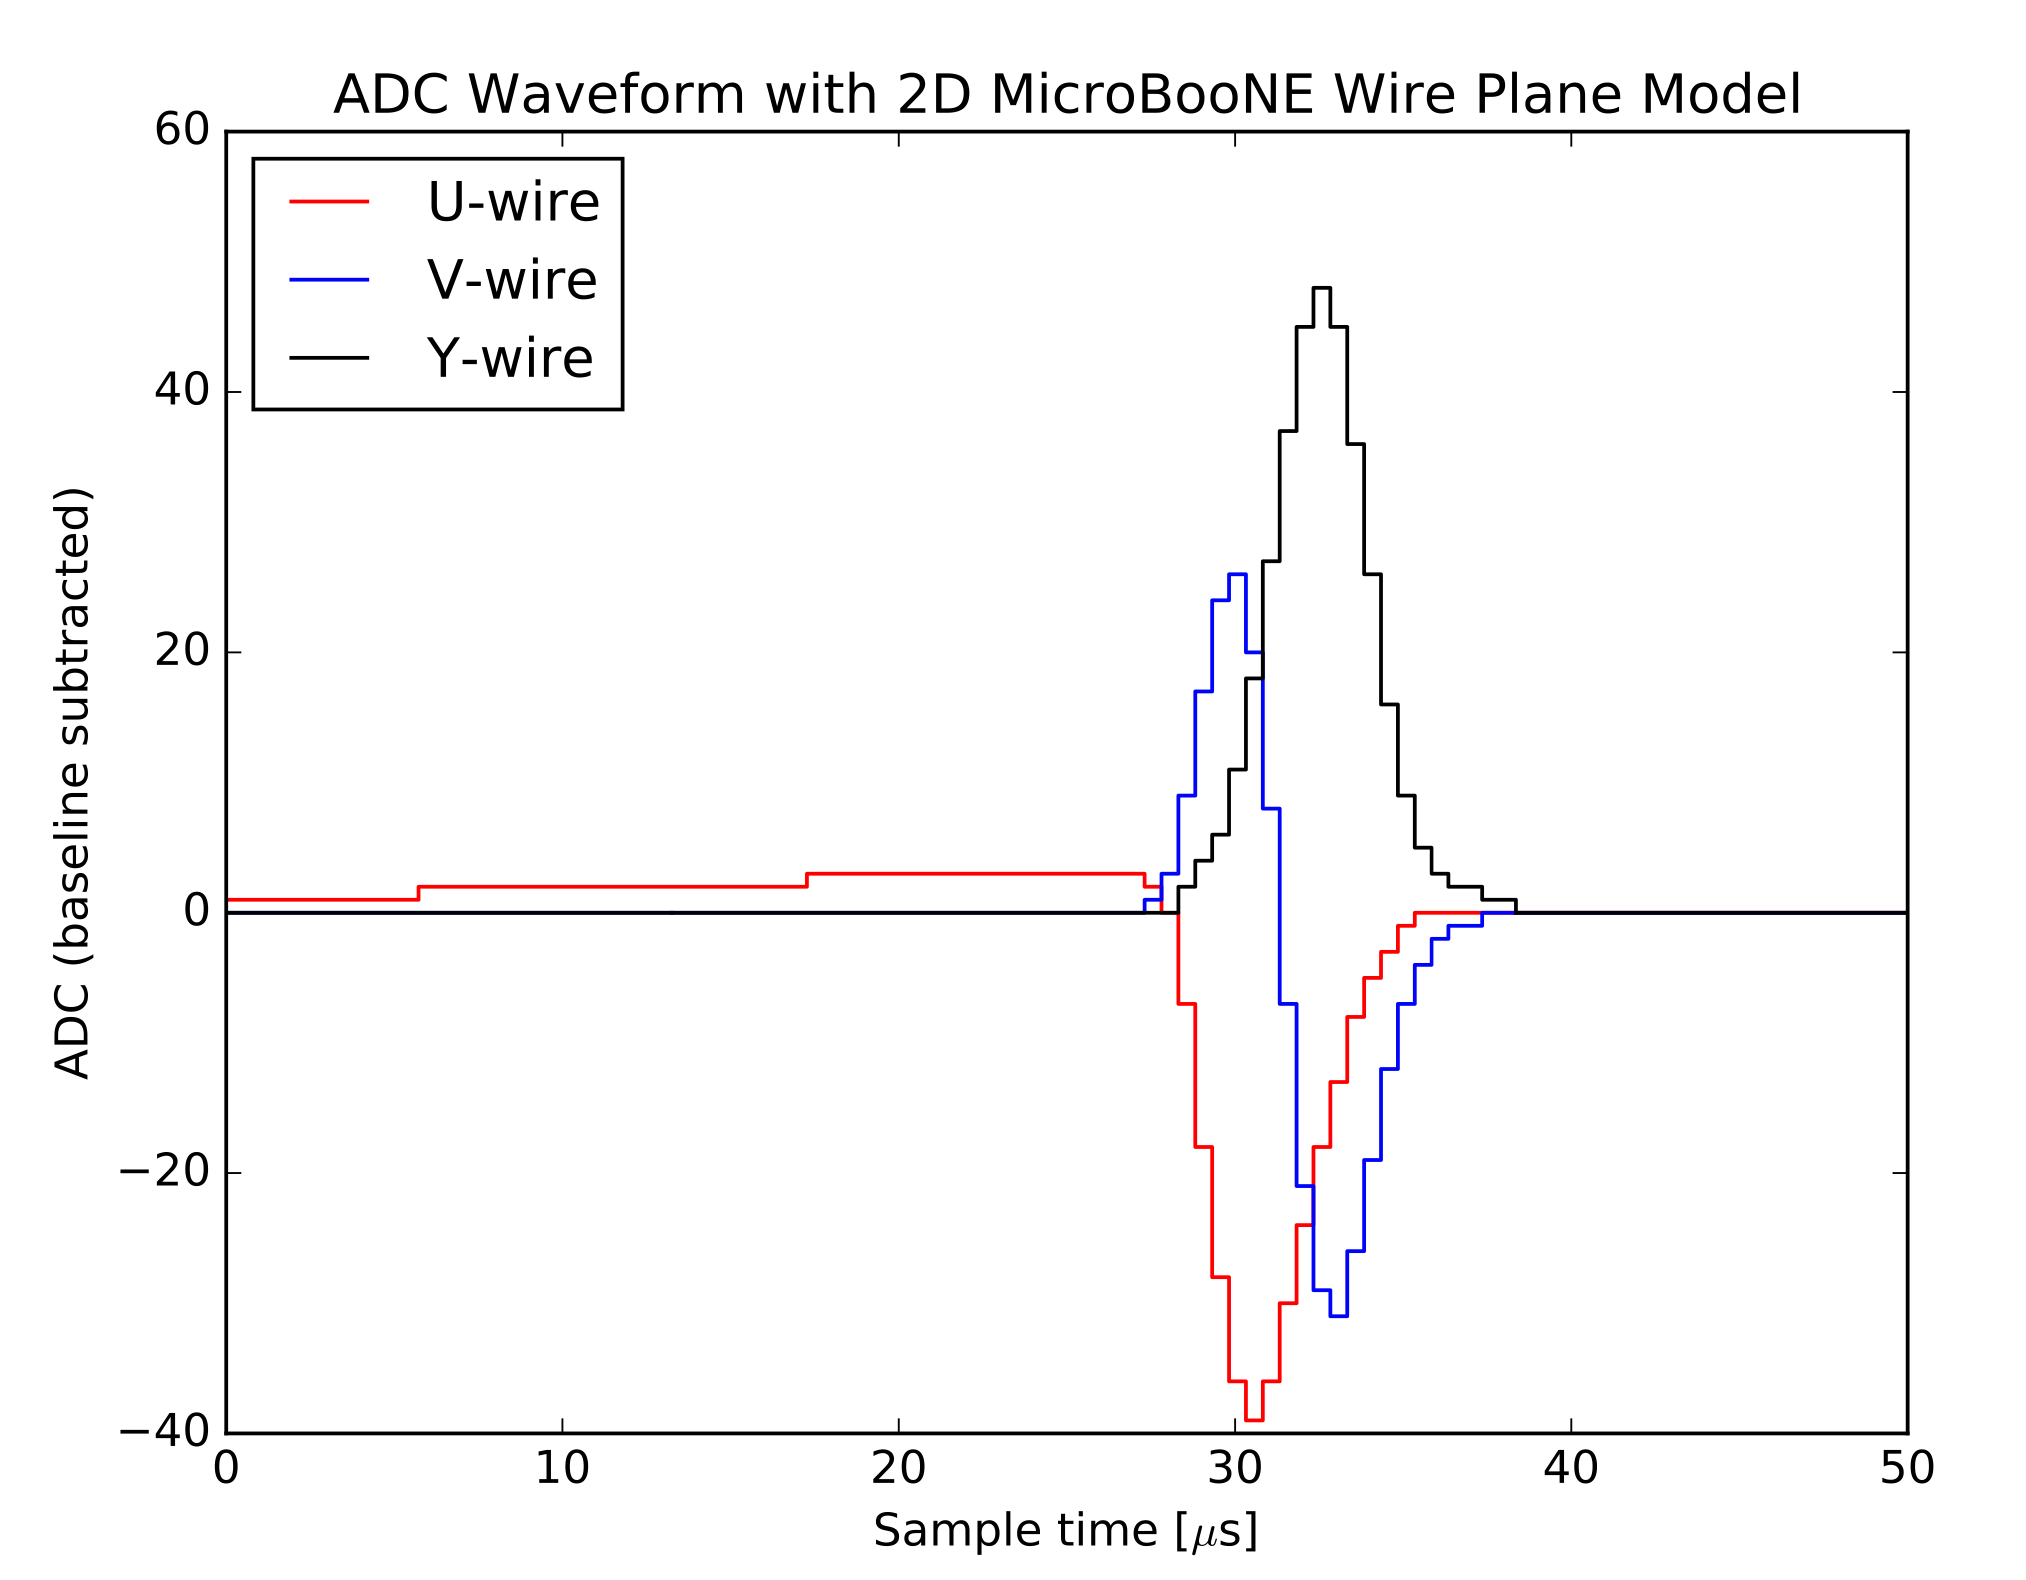
\includegraphics[scale=0.25]{Figures/uboone_dig_signal.png}
		\caption[MicroBooNE's wire planes digital signal]{{\textbf{MicroBooNE's wire planes digital signal}}  \\ Simulation of the digitalized signal of MicroBooNE's wire planes. The U plane corresponds to the induction at $+60^{\circ}$, and the V planes corresponds to the inductin plane at $-60^{\circ}$ and its signal produce takes a bipolar waveform. The Y is the collection plane and its signal takes a unipolar waveform, \cite{microboone_electronics}}
		\label{uboone_digital_signal}	
	\end{center}
\end{figure}

A picture of MicroBooNE's LArTPC assembled can be seen in figure \ref{uboone_lartpc} All three planes have a wire spacing of $3$ mm. The cathode of the LArTPC is at $-70$ V, and the APA is at ground, creating an electric field along the drift direction of $273$ V/cm. At total, MicroBooNE's LArTPC has $8,256$ wires, \cite{microboone_design}. 

\begin{figure}[h!]
	\begin{center}
		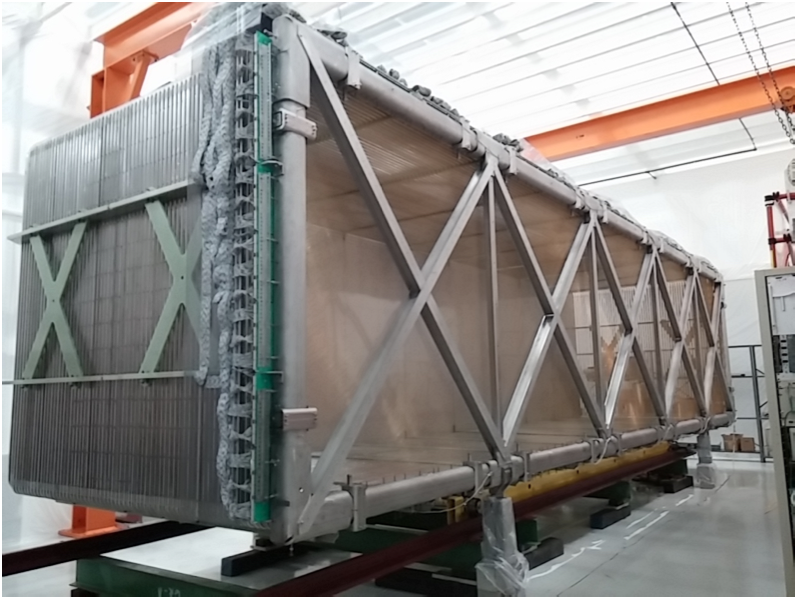
\includegraphics[scale=0.6]{Figures/uboone_LArTPC.png}
		\caption[MicroBooNE's Liquid Argon Time Projection Chamber]{{\textbf{MicroBooNE's Liquid Argon Time Projection Chamber}} \\MicroBooNE's Liquid Argon Time Projection Chamber. The right face is the anode planes face, with the outermost wire plane being the collection plane. \cite{microboone_design}}
		\label{uboone_lartpc}	
	\end{center}
\end{figure}

To keep the argon in liquid form, the LArTPC is immersed in a vessel, called cryostat, that accommodates a total of $170$ ton of Liquid Argon, keeping the temperature at $89$ K and the pressure at $1.2$ atm. How the LArTPC seats inside teh cryostat can be seen in figure \ref{uboone_cryo}.

\begin{figure}[h!]
    \begin{center}
        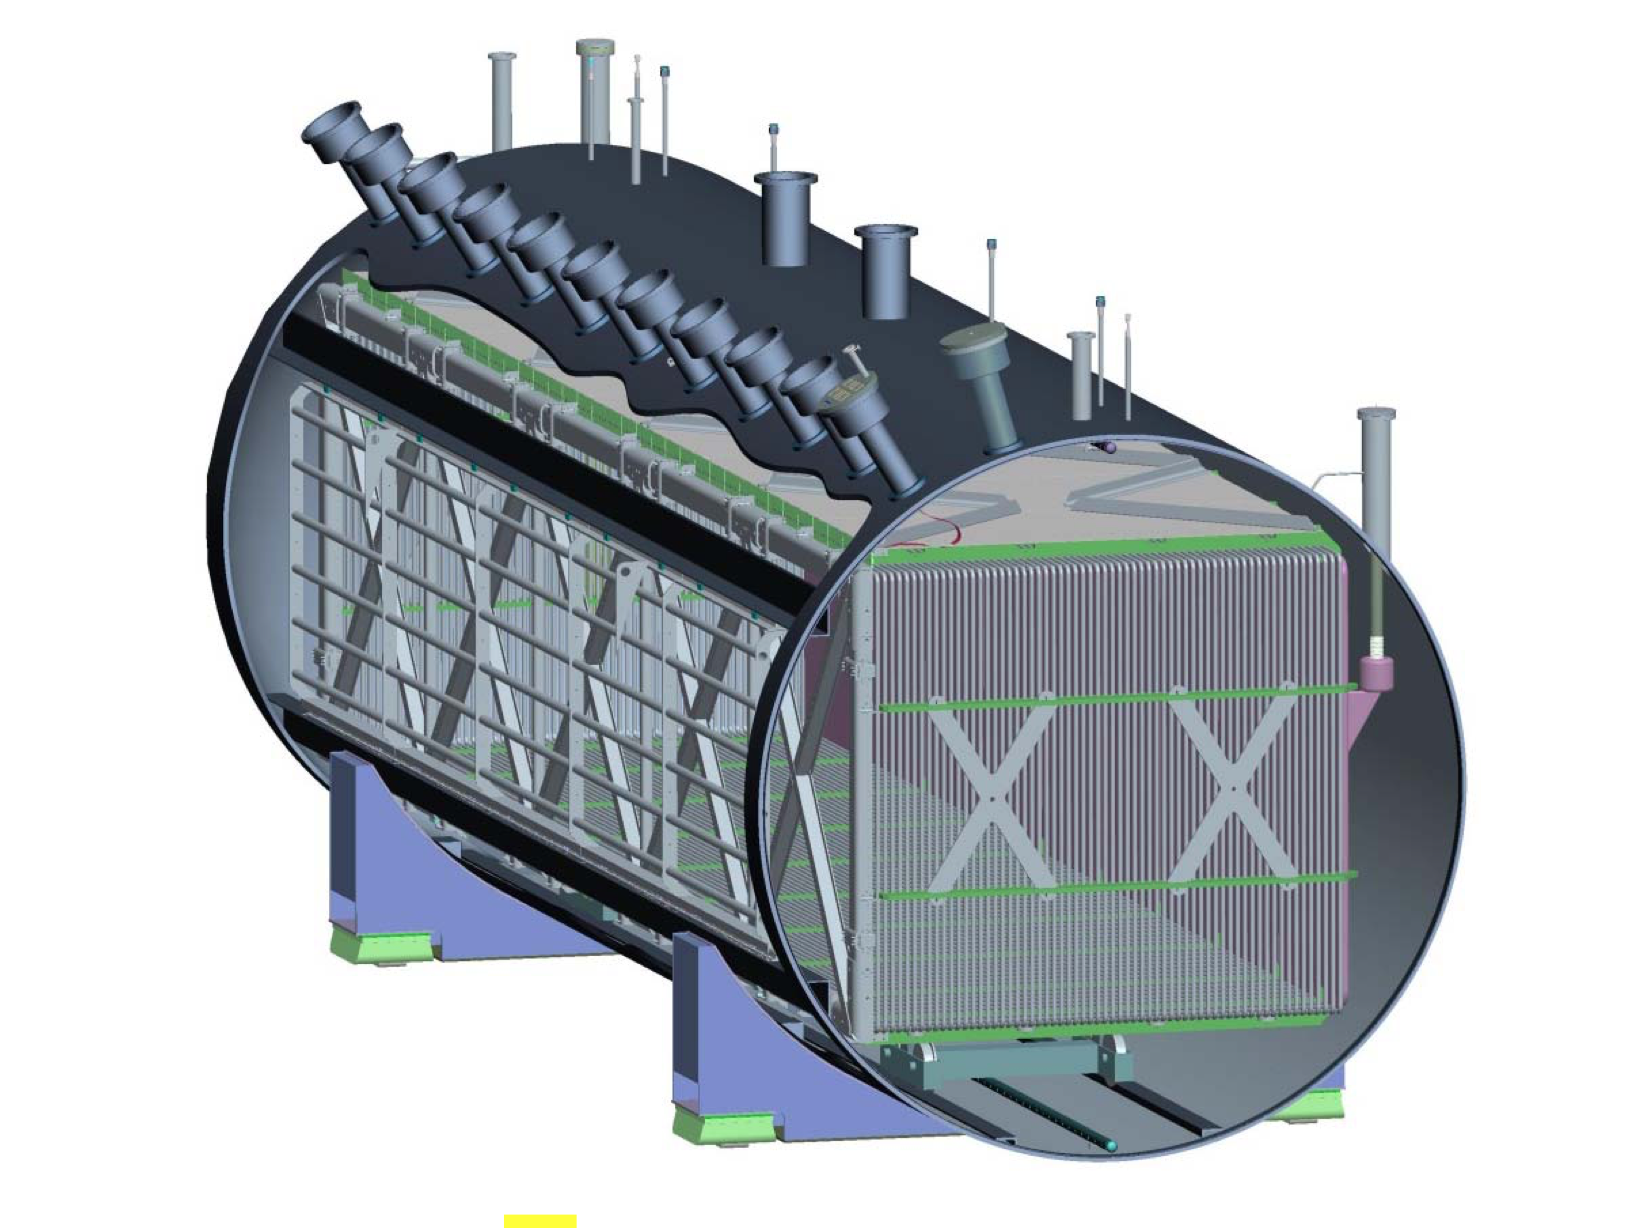
\includegraphics[scale=0.35]{Figures/uboone_cryo.png}
        \caption[MicroBooNE's LArTPC inside the cryostat]{{\textbf{MicroBooNE's LArTPC inside the cryostat}} \\ Schematic view of MicroBooNE's LArTPC inside of the cryostat vessel. The cryostat is the cylindric-like structure in the figure, \cite{microboone_design}.}
        \label{uboone_cryo} 
    \end{center}
\end{figure}

\subsection{Light Collection System}

As mentioned in chapter \ref{Chapter:1}, the scintillation light produced by a charged particle crossing the LArTPC gives the information about the start time of the event. From the difference between the time that the electrons are collected in the collection plane and the start time of the event, plus the knowledge of the drift velocity of the electrons in the detector, we recover the third dimension of the track reconstruction. In MicroBooNE, the drift velocity of the electrons is $1.14$ m/ms. 

This is only possible due to the fact that LAr produces plenty of scintillation light ($\approx 10^4 $) /MeV and that this light is produced and propagated in LAr almost instantaneously ($\approx ns$). The scintillation light is produced in LAr by two mechanisms: self-trapped excitation luminescence and recombination luminescence. Figure \ref{lar-excimers} is a diagram demonstrating those two processes. When a charge particle passes through the liquid argon, it ionizes or excites it. In the first case it will result in light being produced by self-trapped excitation luminescence, which will produce singlet state in $65\%$ of the cases, and a triplet state in $35\%$ of the cases. In the excitation case, it will result in light being produced by recombination luminescence, which will produce singlet states in half of the cases and triplet states in the other half. In all cases the light signal is supressed by impurities in the LAr. Either process produces light with peak at the $128$ nm wavelength, \cite{lar_excimers}.

\begin{figure}[h!]
    \begin{center}
        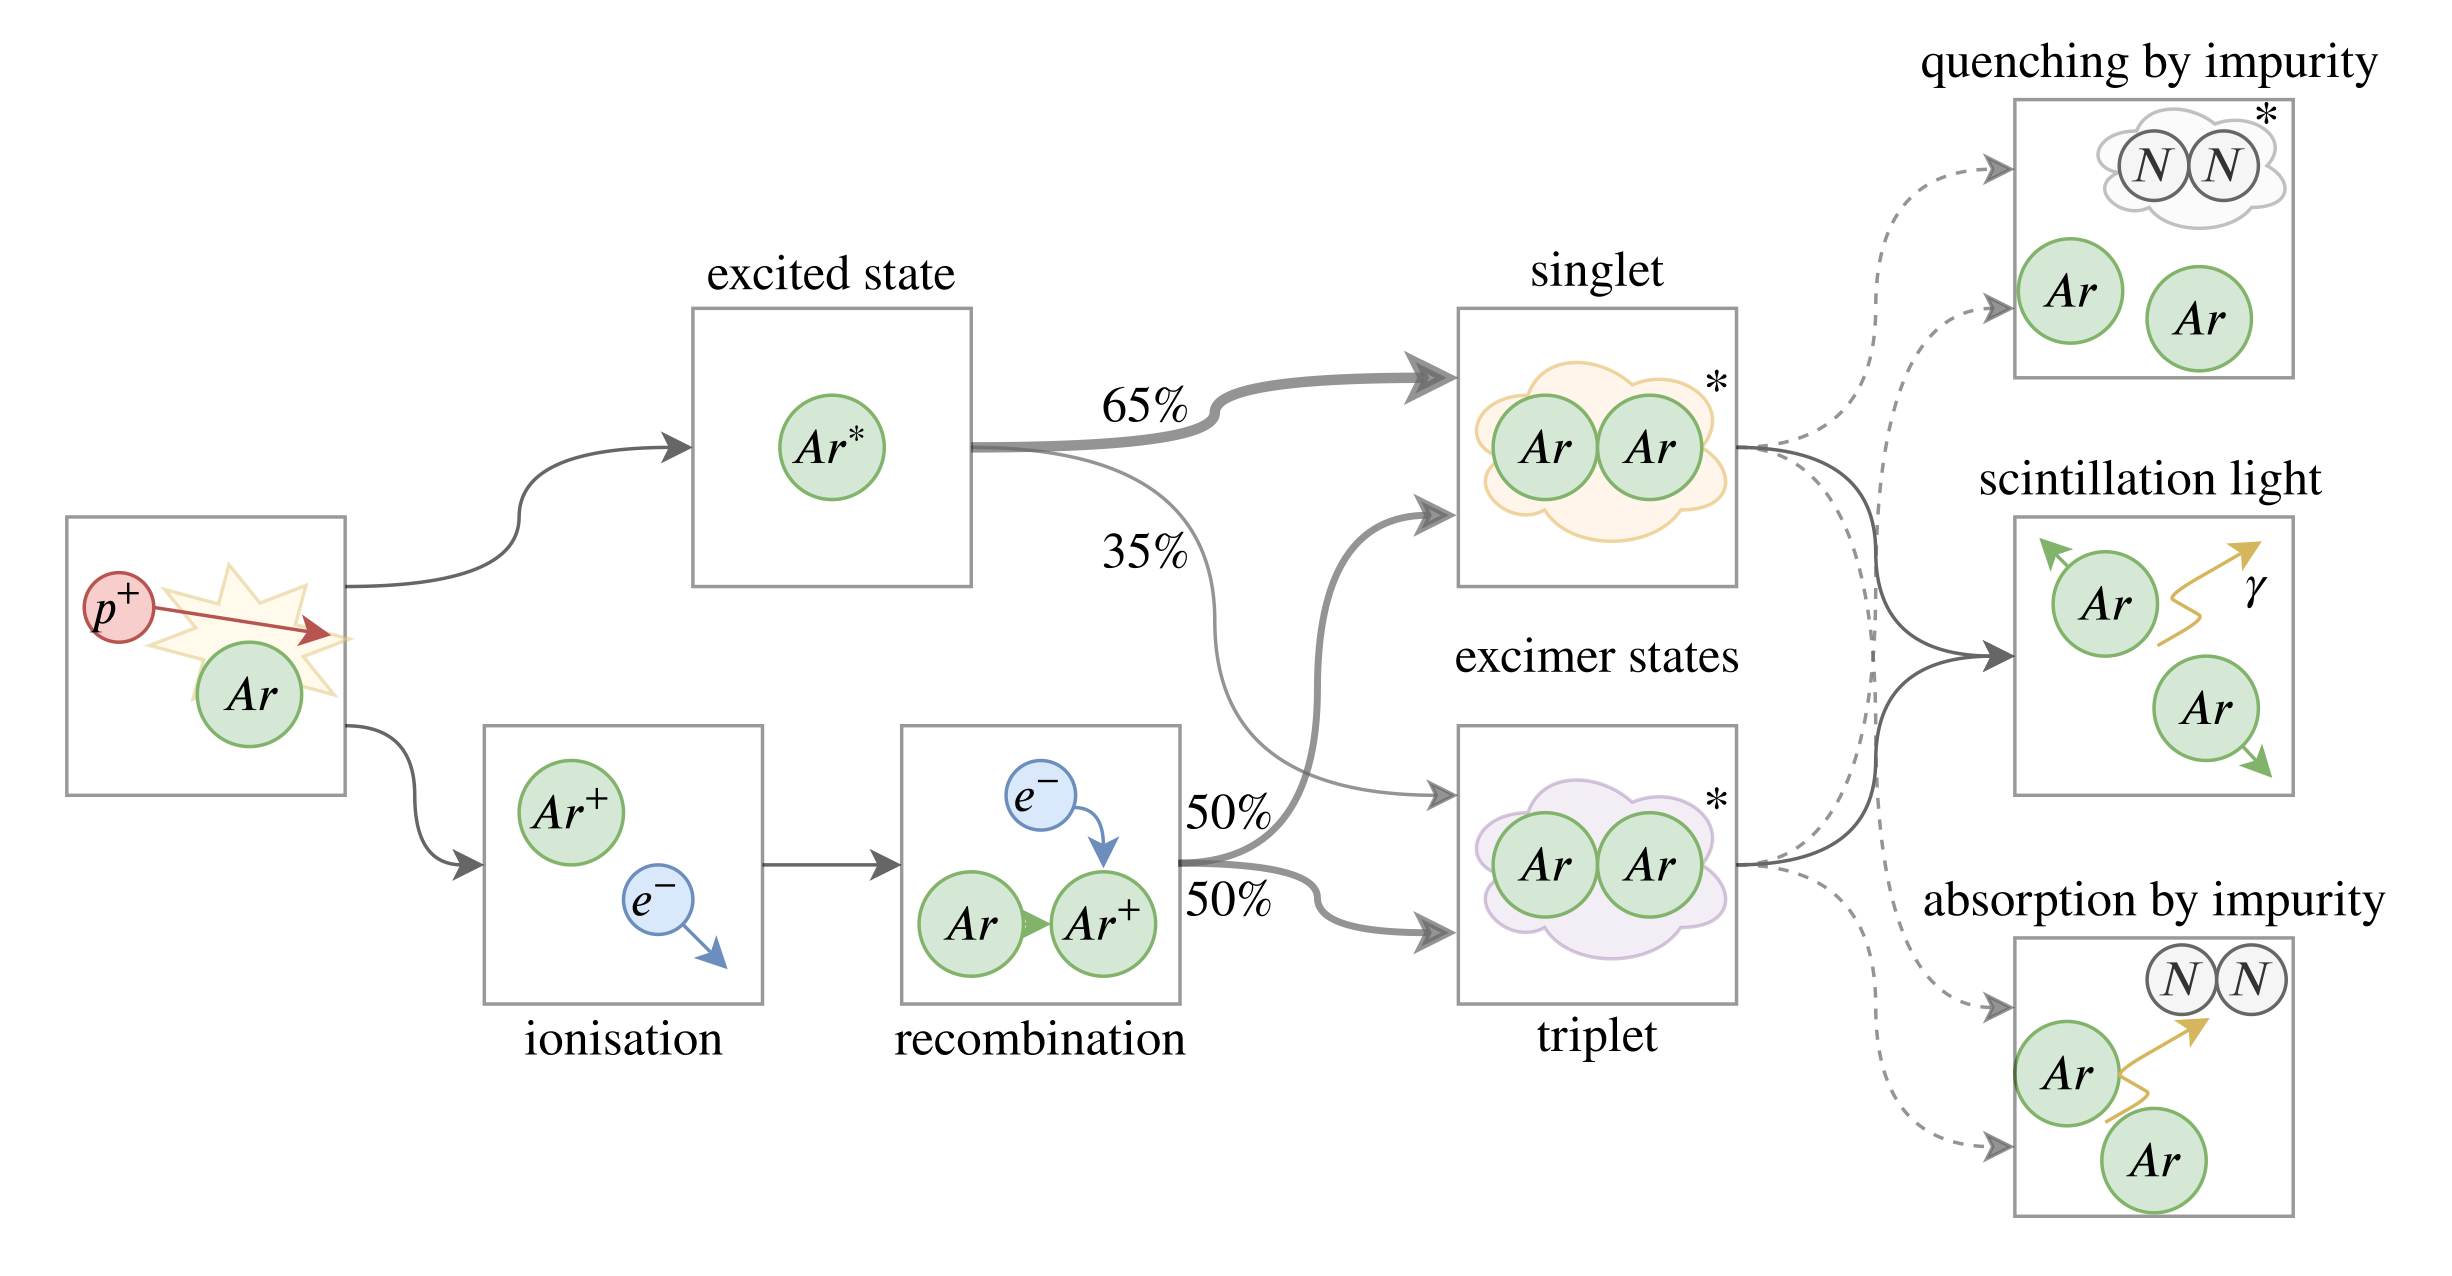
\includegraphics[scale=0.35]{Figures/lar_excimers.png}
        \caption[Scintillation light in liquid argon]{{\textbf{Scintillation light in liquid argon}} When a charge particle passes through the liquid argon, it ionizes or excites it. In the first case it will result in light being produced by self-trapped excitation luminescence In the excitation case, it will result in light being produced by recombination luminescence. In all cases the light signal is supressed by impurities in the LAr. \cite{lar_excimers}.}
        \label{uboone_cryo} 
    \end{center}
\end{figure}

To detect all this light signal, MicroBooNE has $32$ units of 8-inch Hamamatsu photomultiplier tubes (PMTs) arranged behind the APA. Each of them is covered with a plate of tetraphenyl butadiene (TPB) wavelength-shifter, that absorbs the $128$ nm photons and re-emits them at $\approx425$ nm, which is compatible with the PMT's maximum quantum efficiency. A picture of a MicroBooNE PMT is in figure \ref{uboone_pmt}.

\begin{figure}[h!]
    \begin{center}
        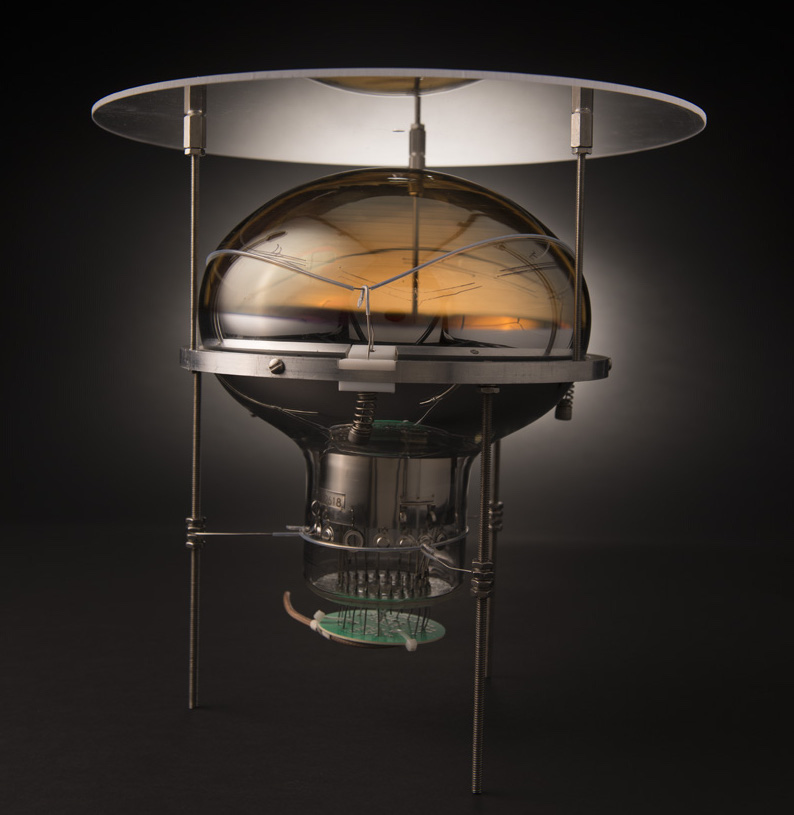
\includegraphics[scale=0.2]{Figures/microboone_pmt.jpeg}
        \caption[MicroBooNE's PMT]{{\textbf{MicroBooNE's PMT}} From: \cite{uboone_pmt}.}
        \label{uboone_pmt} 
    \end{center}
\end{figure}

\section{Neutrino at the Main Injector (NuMI) Beamline}

To study neutrinos, Fermilab artificially produces neutrinos through an accelerator chain that delivers two beams, the Booster Neutrino Beam (BNB) and the Neutrino at the Main Injector (NuMI) beam. Both supply neutrinos to a variety of experiments. MicroBooNE's main beam is the BNB,  but it is also exposed to the NuMI beam. 

The accelerator chain (see full Fermilab's beam chain in \ref{accelerator_chain}) starts with an ion source machine with a molybdenum cathode installed inside of it and filled with hydrogen gas. The molybdenum's electrons are excited and then collected by the hydrogen atoms. The result is a H$^-$ gas. An "extractor" attracts the negative atoms with a positive potential, pulling them through a hole with a width of a few mm, while a magnetic field guides them in the right direction to feed the beam into a radio-frequency quadrupole (RFQ). The RFQ receives the low-energy beam from the ion source at one end and injects a $750$ keV \cite{RFQ_website} beam into the other end, delivering it to a linear accelerator (LINAC). The LINAC is $150$ m  long and is divided into two acceleration parts. The first is a drift tube that accelerates the beam up to $116$ MeV, and the second is a side-coupled cavity that accelerates the beam up to $401$ MeV \cite{LINAC_website}. Exiting the LINAC, the beam collides with a thin carbon sheet that removes electrons from the H$^-$, resulting in three beams: a $H^-$ beam, a $H^+$ beam, and a $H^0$ beam. Only the pure proton beam is selected. After all this process, the beam is suitable to be inserted into a circular $75$ m radius accelerator called Booster, which extracts a beam of $8$ GeV protons that can be directed towards the Main Injector (MI), the BNB target, or to the Recycler \cite{booster_website}. For the NuMI beam, the protons from the Booster are directed towards a $3319.4$ m circumference synchrotron, called the Main Injector, that further accelerates the protons up to $120$ GeV. Those protons are then directed towards a graphite target, where they collide, producing the NuMI beam.

\newpage
\begin{figure}[h!]
	\begin{center}
		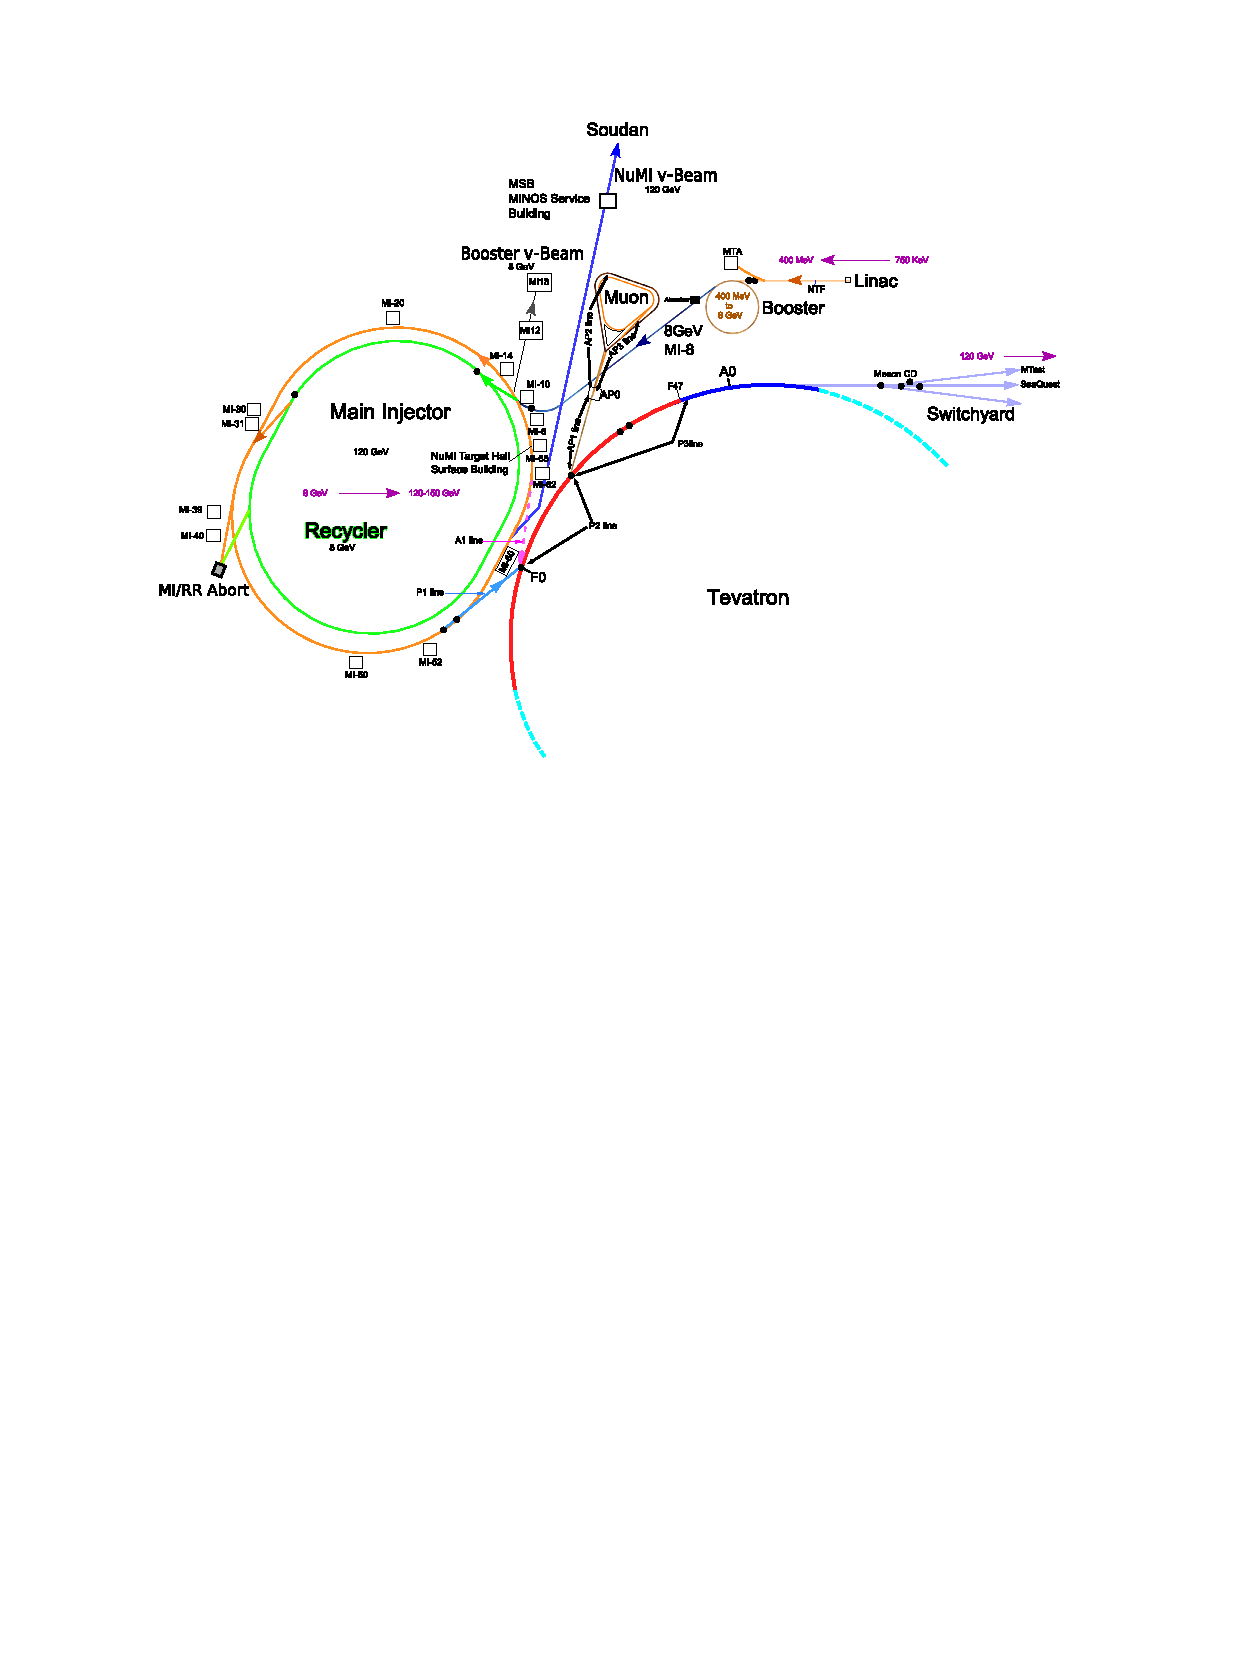
\includegraphics[scale=0.8]{Figures/acceleratorChain.pdf}
		\caption[Full Fermilab's beam chain]{ {\textbf{Full Fermilab's beam chain}} \\ The image shows the Fermilab beam chain map, from the RFQ/LINAC to the main injector, BNB, or to the recycler, \cite{paper_numibeamline}.}
		\label{accelerator_chain}	
	\end{center}
\end{figure}
%

In the NuMI beam, when the $120$ GeV protons are thrown at a graphite target, they produce mesons. These mesons are focused by magnetic horns and directed to the $675$ m long decay pipe, where they decay into muons and muon-neutrinos, as shown in the schematic view of the beamline in figure \ref{fig:numi}. After the decay pipe, an absorber blocks the remaining hadrons and muons in the beamline, leaving a pure neutrino beam beyond it. 

\begin{figure}[h!]
    \centering
    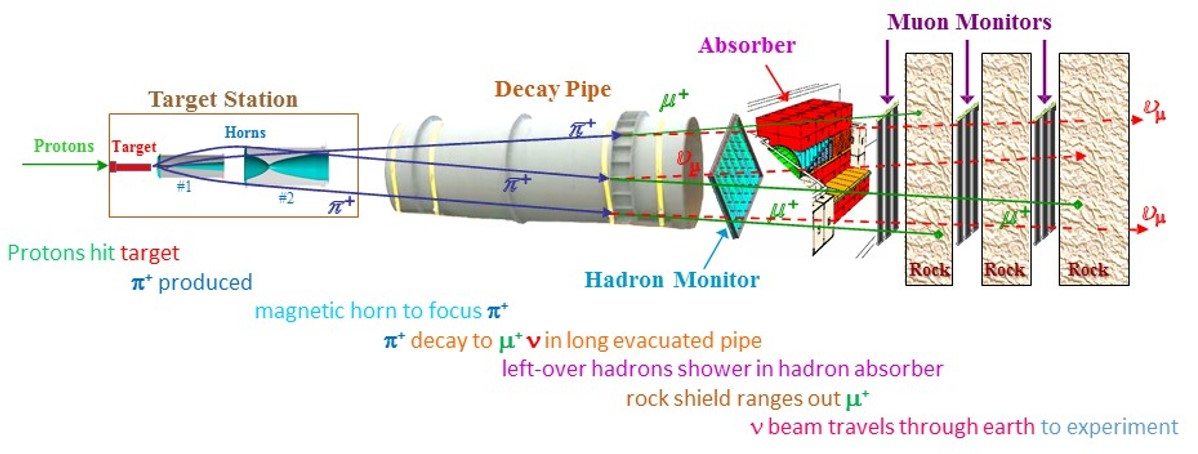
\includegraphics[width=140mm]{Figures/numi.jpg}
    \caption{NuMI layout \cite{numi}.}
    \label{fig:numi}
\end{figure}

By changing the polarity of the magnetic horns, we can select the sign of the charged mesons. By having positive horn current, we select positive particles. We call it the Forward Horn Current (FHC) mode, or Neutrino Mode. By having negative horn current, we select negative particles. We call it the Reverse Horn Current (RHC) mode, or Antineutrino Mode. In figure \ref{beam_mode_uboone} you can find a plot of the number of Protons on Target (POT) delivered in each run of MicroBooNE and in which mode the beam was selected. The NuMI beam delivers neutrinos in windows of $9.6 \mu$ s. During MicroBooNE's operation time we collected a total of $2.3\times 10^{21}$ POT, $1.0\times10^{21}$ in Neutrino Mode and $1.3\times10^{21}$ in Antineutrino Mode

\begin{figure}[h!]
    \centering
    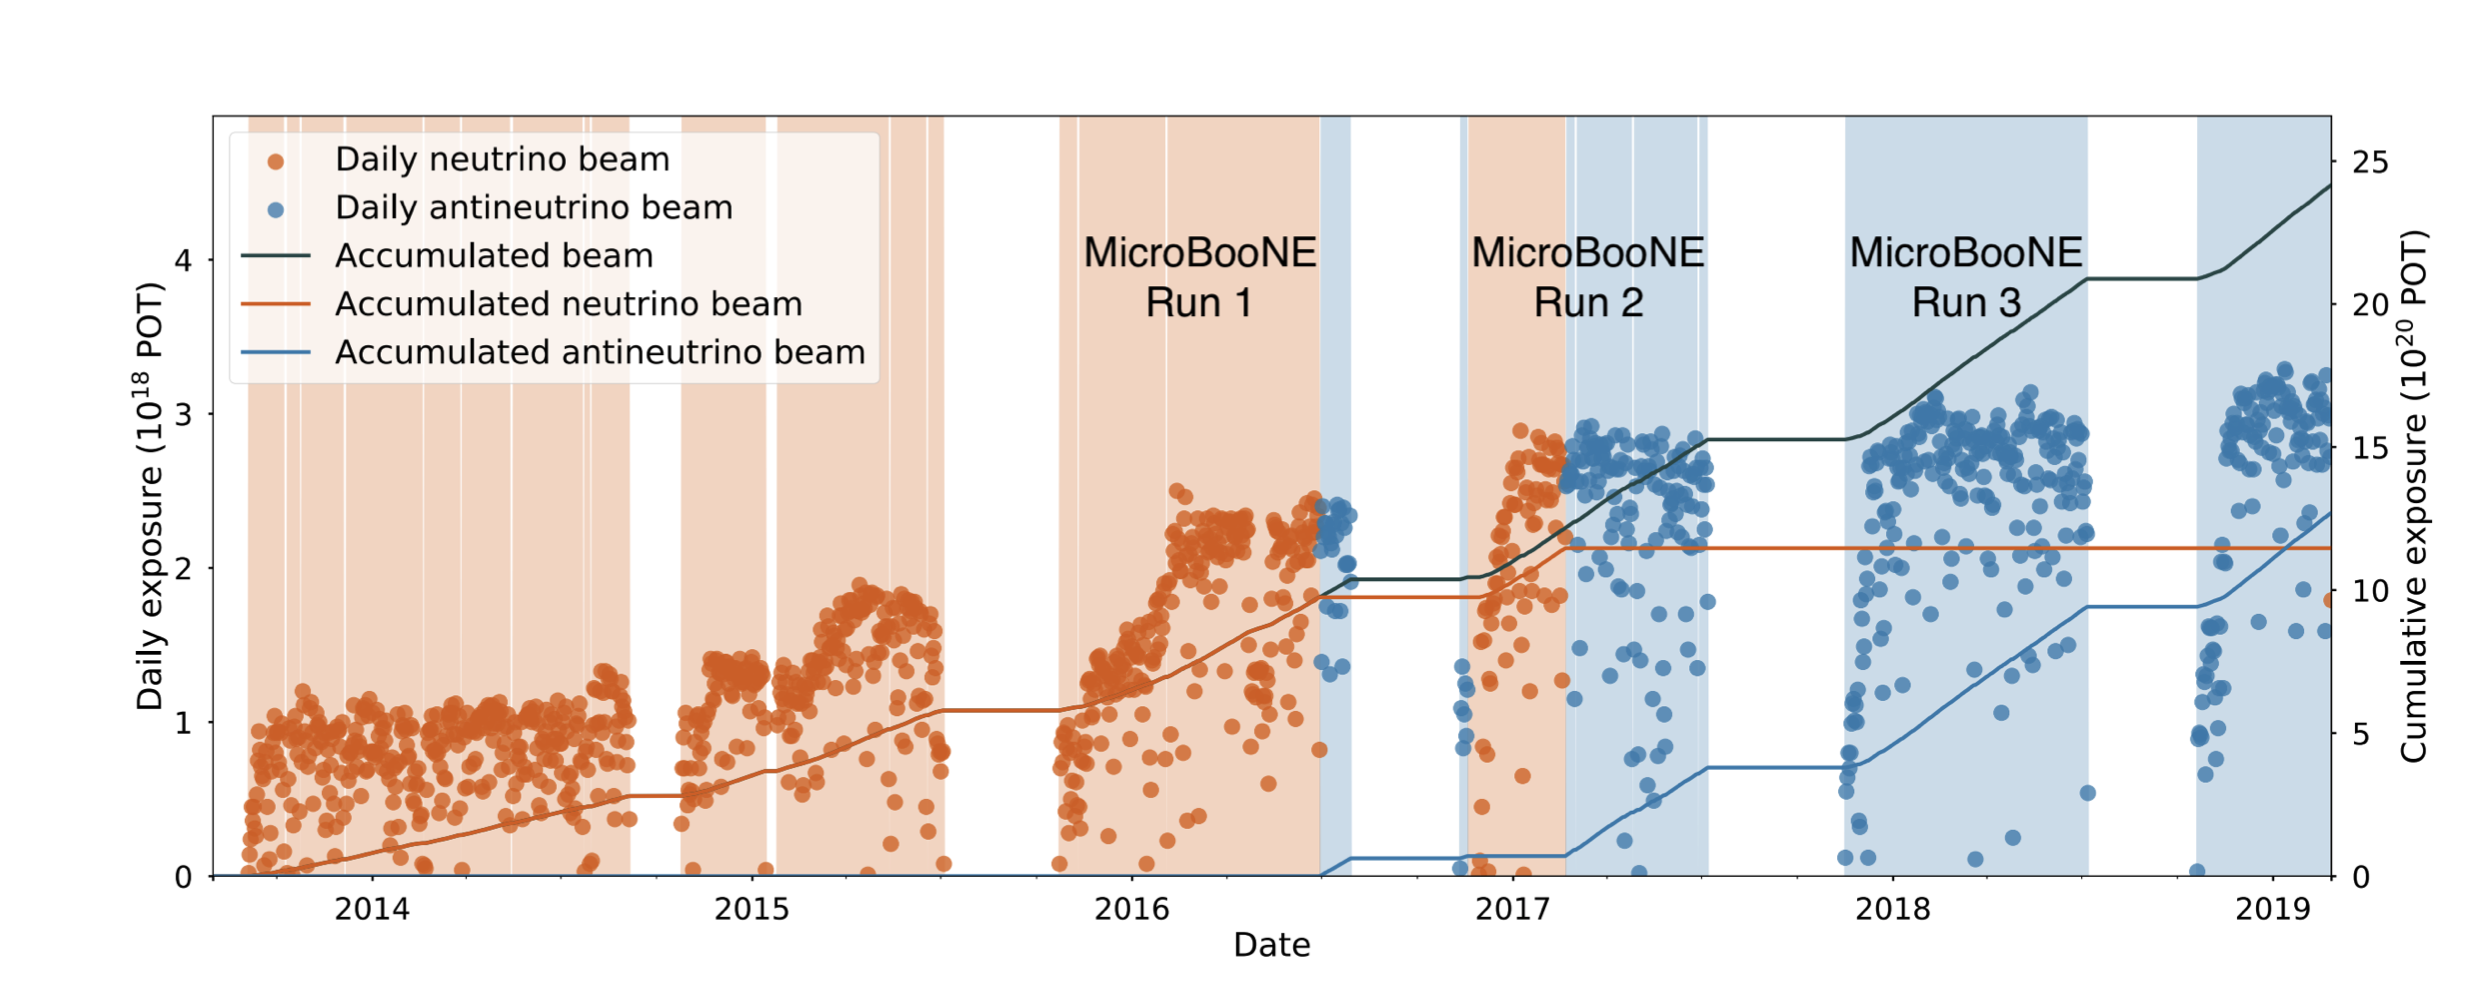
\includegraphics[width=150mm]{Figures/beam_mode_uboone.png}
    \caption{The cumulative POT from NuMI delievered to MicroBrooNE. In the orange regions the horn polarity was in Neutrino Mode. In the blue regions the horn polarity was in Antineutrino Mode. The white regions refer to periods in which the accelerator complex was shut down. \cite{krish_phd}.}
    \label{beam_mode_uboone}
\end{figure}

\section{MicroBooNE's Data Acquisition and Processing}